\section{Virtual Memory Management}

Bei der virtuellen Speicherverwaltung erfolgt die Umwandlung von vom ARM Prozessor generierten, virtuellen Adressen in physikalische Adressen durch die \emph{Memory Management Unit} (MMU). Dieses Kapitel enthält die Beschreibung des Designs und der Implementierung der virtuellen Speicherverwaltung des Betriebssystems sowie der Einstellungen der MMU.\\

\subsection{Grundlegende Funktionsweise}

Die \emph{VSMAv7} definiert zwei unabhängige Formate für translation tables \cite[S. B3-1318]{ARM:ARM}:

\begin{itemize}
	\item \emph{Short-descriptor format}:
	\begin{itemize}
		\item zweistufige Seitentabelle 
		\item 32-bit Deskriptoren (PTE)
		\item 32-bit virtuelle Eingangsadresse 
		\item bis zu 40-bit große physikalische Ausgangsaddresse
	\end{itemize}
	\item \emph{Long-descriptor format}:
	\begin{itemize}
		\item dreistufige Seitentabelle
		\item 64-bit Deskriptoren (PTE)
		\item verwendet \emph{Large Physical Address Extension} (LPAE)
		\item bis zu 40-bit große virtuelle Eingangsadresse 
		\item bis zu 40-bit große physikalische Ausgangsaddresse
	\end{itemize}
\end{itemize}

Um die Anforderungen an das Betriebssystem zu erfüllen, reicht das zweistufige Seitentabellensystem vollkommen aus. Tabelle \ref{table:GeneralVirtualMemory} fasst die wichtigsten gegebenen Eigenschaften unter Verwendung des Short-descriptor format zusammen.\\

\begin{table}[H]
\begin{tabular}{p{7cm} | p{7cm}}
  \textbf{Eigenschaft} & \textbf{Beschreibung} \\ \hline
  Virtueller Speicher & 4 GB\\  
  Größe eines Page Table Entry (PTE) & 4 Byte \\
  Einträge L1 Page Table & 4096\\
  Einträge L2 Page Table & 256\\
  Speicherbedarf L1 Page Table & 4 Byte * 4096 = 16kB \\
  Speicherbedarf L2 Page Table & 4 Byte * 256 = 1kB\\
  Unterstützte Pagegrößen: & \emph{small page} (4 kB), \emph{large page} (64 kB)\\
  Unterstützte Sectiongrößen: & \emph{section} (1 MB), \emph{supersection} (16 MB)\\
 \end{tabular}
 \caption{Eigenschaften der virtuellen Speicherverwaltung der ARMv7-Architektur}
 \label{table:GeneralVirtualMemory}
\end{table}

Generiert die ARM CPU einen Speicherzugriff, wird von der MMU ein Suchlauf durchgeführt. Dieser Suchlauf wird \emph{translation table lookup} genannt. Dabei wird zuerst im Translation Lookaside Buffer (\emph{TLB}) nachgesehen, ob einer der 64 Einträge des TLB die zur virtuellen Adresse korrespondierente physikalische Adresse enthält. Ist dies der Fall (so genannter \emph{TLB hit}), wird der Suchlauf an dieser Stelle erfolgreich beendet.\\

Ist die angeforderte virtuelle Adresse nicht im TLB enthalten (TLB miss), wird ein page table walk durchgeführt. Das Funktionsprinzip des zweistufigen Seitentabellensystems zeigt Abbildung \ref{fig:2levelTableSystem}. Aus einem der zwei Seitentabellenregister wird die Basisadresse der darin zuvor abgelegten L1-Seitentabelle geholt. Das Format der \emph{page table entries (PTE)} bestimmt dann, um welchen Typ von Verweis es sich handelt. Seitentabellen und ihre Einträge werden im nachfolgenden Abschnitt \ref{subsect:pageTables} genauer beschrieben.\\

\begin{figure}[H]
	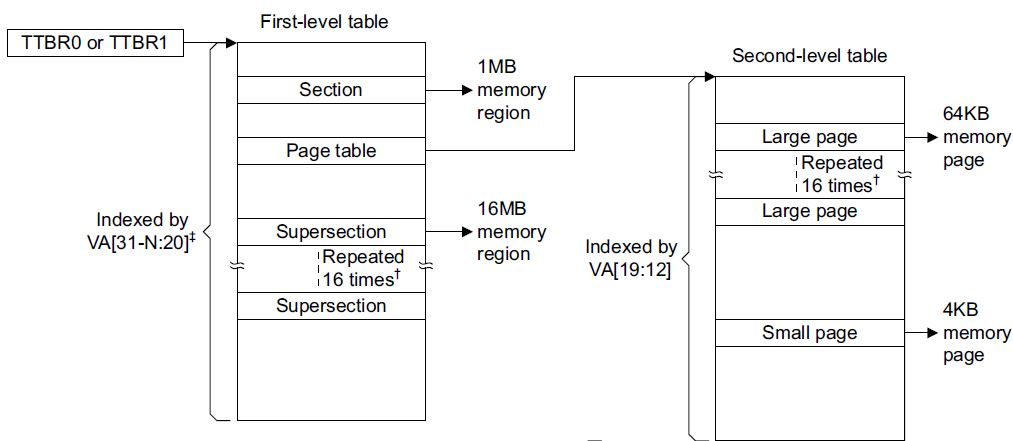
\includegraphics[scale=0.7]{figures/addressTranslation}
	\caption{Zweistufiges Seitentabellensystem \cite[S. B3-1325]{ARM:ARM}}
	\label{fig:2levelTableSystem}
\end{figure}

\vspace{2cm}
DATA ABORT HANDLER BESCHREIBEN
\vspace{2cm}

\subsection{Umwandlung virtueller Adressen zu physikalische Adressen}

Der genaue Vorgang der Umwandlung einer vom ARM Prozessor erzeugten virtuellen Adresse in eine physikalische Speicheradresse zeigen die nachfolgenden beiden Abbildungen. Abbildung  \ref{fig:sectionTranslation} zeigt die Umwandlung einer virtuellen Adresse in die physikalische Adresse einer 1 MB Section ohne Verwendung einer L2-Seitentabelle, Abbildung \ref{fig:smallPageTranslation} diejenige einer virtuellen Adresse in ein 4 kB page frame unter Verwendung einer L2-Seitentabelle.   Die Umwandlung wird vollständig durch die Prozessor-Hardware durchgeführt.\\


\begin{figure}[H]
	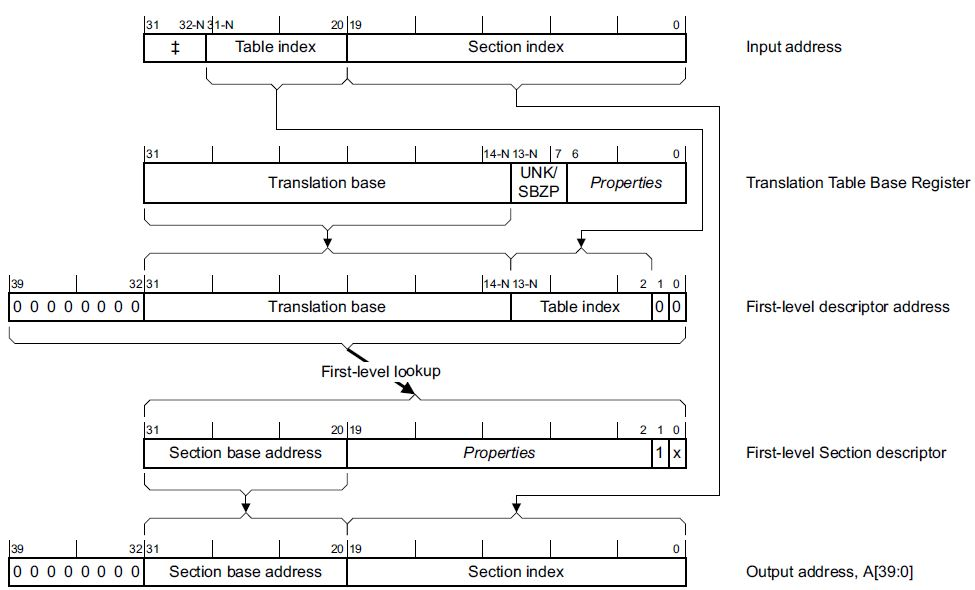
\includegraphics[scale=0.8]{figures/sectionTranslation}
	\caption{1 MB Section Translation durch die ARM CPU \cite[S. B3-1335]{ARM:ARM}}
	\label{fig:sectionTranslation}
\end{figure}

\begin{figure}[H]
	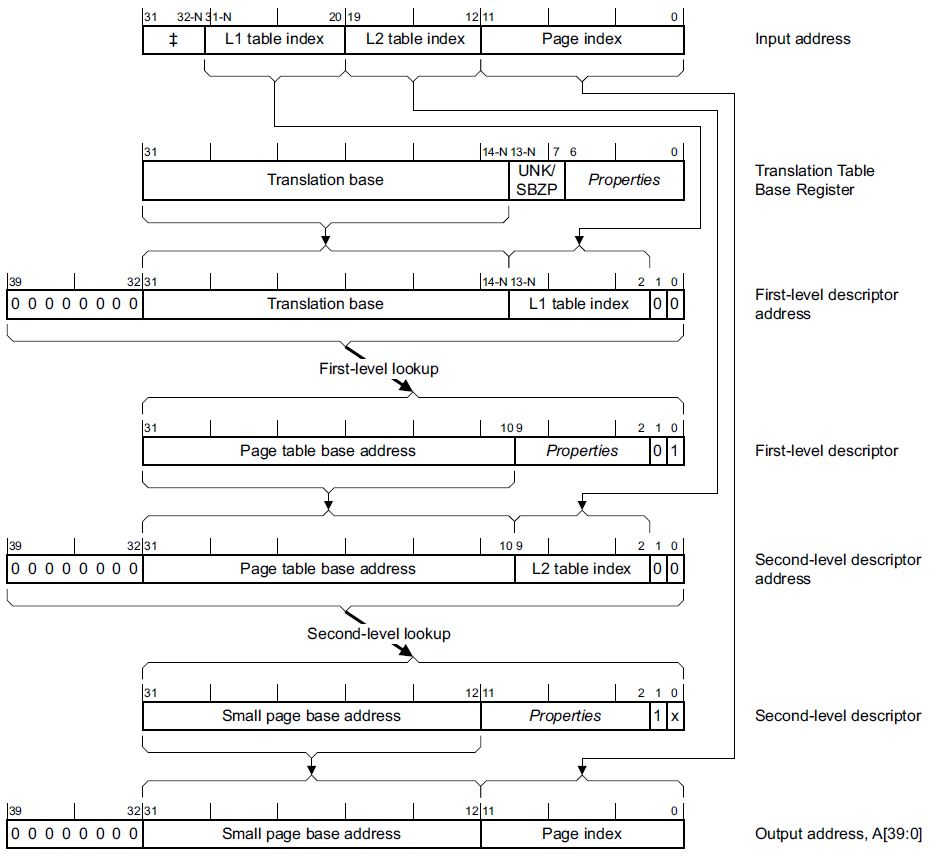
\includegraphics[scale=0.8]{figures/smallPageTranslation}
	\caption{Small Page Translation durch die ARM CPU \cite[S. B3-1337]{ARM:ARM}}
	\label{fig:smallPageTranslation}
\end{figure}

\subsection{Seitentabellen und Seitentabelleneinträge}
\label{subsect:pageTables}

Der verwendete ARM Prozessor verfügt über zwei Register (\emph{Translation Table Base Register}, \emph{TTBR0} und \emph{TTBR1}), welche Startadressen von Seitentabellen enthalten  \cite[S. B3-1320]{ARM:ARM}. Ihre Formate sind nahezu identisch und in den Abbildungen \ref{fig:TTBR0Format} und \ref{fig:TTBR1Format} zu sehen. Diese Register übernehmen im Betriebssystem die folgende Funktion:

\begin{itemize}
	\item TTBR0: Wird für prozessspezifische Adressen verwendet. Jeder Prozess enthält bei seiner Initialisierung eine eigene L1-Seitentabelle. Bei einem Kontextwechsel erhält das TTBR0 eine Referenz auf L1-Seitentabelle des neuen Kontextes/Prozesses.
	\item TTBR1: Wird für das Betriebssystem selbst und für memory-mapped I/O verwendet. Diese ändern sich bei einem Kontextwechsel nicht.
\end{itemize}


\begin{figure}[H]
	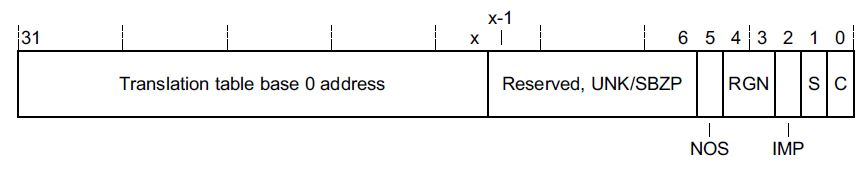
\includegraphics[scale=0.8]{figures/ttbr0format}
	\caption{TTBR0 Format \cite[S. B4-1726]{ARM:ARM}}
	\label{fig:TTBR0Format}
\end{figure}


\begin{figure}[H]
	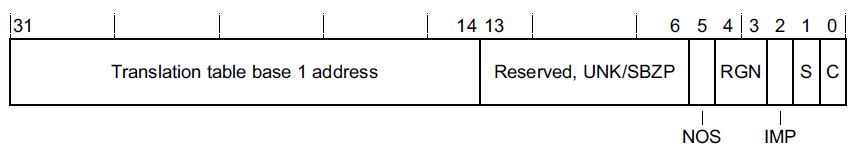
\includegraphics[scale=0.8]{figures/ttbr1format}
	\caption{TTBR1 Format \cite[S. B4-1730]{ARM:ARM}}
	\label{fig:TTBR1Format}
\end{figure}

Das Beschreiben der Seitentabellenregister erfolgt, wie bei nahezu jeder MMU-Funktionalität, mittels Assemblerbefehlen, die auf die CP15 Coprozessor Register zugreifen.\\

Beim Füllen der Seitentabllen sind vorgegebene Formate für die beiden Typen von Deskriptoren unbedingt zu beachten. Die Abbildungen \ref{fig:firstLevelDescriptor} und \ref{fig:secondLevelDescriptor} fassen die Formate für first-level und second-level Deskriptoren zusammen. Beiden Deskriptortypen gleich ist der Fehlereintrag, der aus nullen besteht.\\

\subsubsection*{First-level Deskriptoren}

Die First-Level Deskriptortypen werden auf folgende Weise verwendet:

\begin{itemize}
	\item sections für die master page table (siehe Abschnitt \ref{subsect:memoryMapping}) 
	\item page table für L1-Seitentabellen von Prozessen (siehe Abschnitt \ref{subsect:memoryMapping})
\end{itemize}

\begin{figure}[H]
	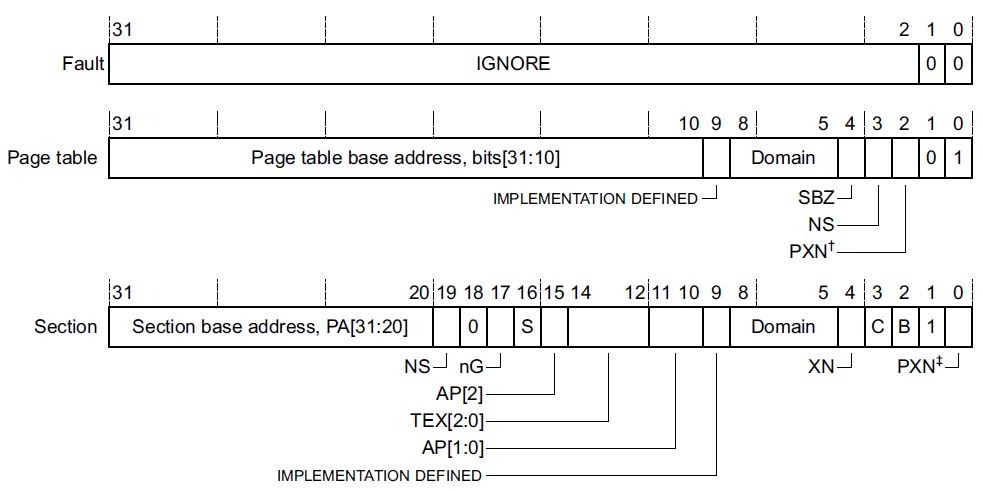
\includegraphics[scale=0.7]{figures/firstLevelDescriptor}
	\caption{First-Level Deskriptorformate \cite[S. B3-1326]{ARM:ARM}}
	\label{fig:firstLevelDescriptor}
\end{figure}

\subsection*{Second-level Deskriptoren}

In der Speicherverwaltung des Betriebssystems werden ausschließlich small pages verwendet. Ausschlaggebende Gründe, warum small pages den Vorzug gegenüber large pages erhielten, sind die folgenden:

\begin{itemize}
	\item small pages müssen nur einmal in die L2-Seitentabelle eingetragen werden, large pages hingegen 16 mal
	\item L1- und L2-Seitentabellen, die 16 kB bzw. 1 kB Speicher benötigen, belegen bei ihrer Erzeugung nur vier volle page frames bzw. ein page frame physikalischen Speichers zu einem Viertel. Dadurch wird die Speicherfragmentierung vergliechen mit large pages stark verringert
\end{itemize}

\begin{figure}[H]
	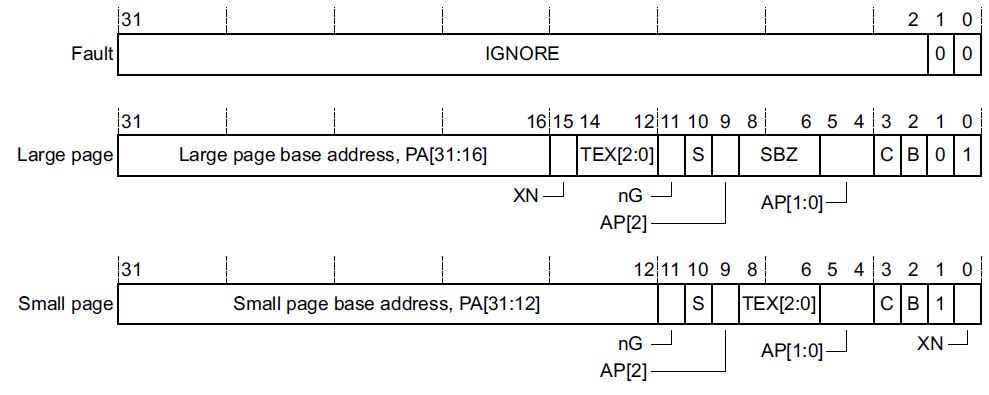
\includegraphics[scale=0.7]{figures/secondLevelDescriptor}
	\caption{Secondt-Level Deskriptorformate \cite[S. B3-1327]{ARM:ARM}}
	\label{fig:secondLevelDescriptor}
\end{figure}

\subsection{Aufteilung des virtuellen Speichers und Mapping}
\label{subsect:memoryMapping}

Die Speicherverwaltung des Betriebssystems kann Abbildung \ref{fig:MemoryMap} entnommen werden. Die rechte Seite stellt das physikalische Speichermapping dar und wurde dem Datenblatt des ARM \cite[S. 155]{ARM:TRM} entnommen. Die linke Seite zeigt die Aufteilung des virtuellen Speichers.\\

Organisiert ist der virtuelle Speicher in Speicherregionen. Eine zusätzliche Aufteilung betrifft die Zuständigkeitsbereiche für die Seitentabellenregister TTBR0 und TTBR1. Im Seitentabellenkontrollregister TTBCR (Translation Table Base Control Register, \cite[S. B4-1721]{ARM:ARM}) können den Seitentabellenregistern Adressbereiche zugewiesen werden.

Physikalisch steht 1 GB Speicher für die page frames zur Verfügung.

Komponenten, die sich bei einem Kontextwechsel nicht ändern, werden statisch in master page table gemappt. Dazu zählen memory mapped I/O, Kernel des Betriebssystems, die Adressen der Exceptionhandler sowie die page table region, in welcher die L1- und L2-Seitentabellen abgelegt werden. Diese Komponenten befinden sich an den Adressen von 0x40000000 bis 0x81500000 und werden in die master page table direkt, d.h. Eins-zu-eins, gemapped. Ein Zugriff auf eine virtuelle Adresse ergibt damit einen Zugriff auf dieselbe Adresse in physikalischen Speicher.

Der Adressbereich von 0x00000000 bis 0x40000000 entspricht genau 1 GB. In ihn wird der virtuelle Prozessbereich an diese Adressen gemapped und somit 0x40000000 als Selektionsgrenze zwischen TTBR0 (für Prozesse) und TTBR1 (für Kernelfunktionen) festgelegt.

Die master page table wird bei der Initialisierung der MMU im TTBR1 abgelegt. Danach wird der Inhalt des TTBR1 während der Laufzeit des Betriebssystems nie wieder aktualisiert bzw. geändert.

Bei der Initialisierung eines Prozesses wird für den Prozess eine L1-Seitentabelle, die mit Fehlereinträgen initialisiert ist, angelegt. Soll ein Prozess zur Ausführung gebracht werden, muss seine L1-Seitentabelle in das TTBR0 geschrieben werden. Das TTBR0 muss zur Laufzeit des Betriebssystems bei Kontextwechseln von Prozessen aktualisiert werden.





\begin{figure}[H]
	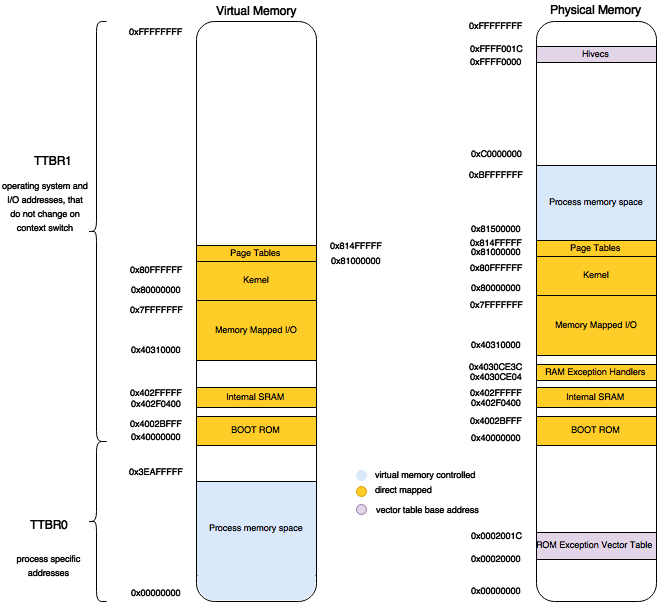
\includegraphics[scale=0.7]{figures/MemoryMap}
	\caption{Memory Map des Betriebssystems}
	\label{fig:MemoryMap}
\end{figure}

\begin{table}[H]
\begin{tabular}{p{7cm} | p{7cm}}
  \textbf{Eigenschaft} & \textbf{Beschreibung} \\ \hline
  Größe der Pages & 4 kB\\
  Speicherbedarf Kernel & 16 MB\\
  Virtueller Speicher für Prozesse & 1003 MB\\
  Physikalischer Speicher für Page Tables	& 5 MB\\
  Max. Anzahl von L1 und L2 Page Tables & 320 L1 Page Tables oder 1 L1 Page Table + 1276 L2 Page  Table\\
  Theoretisch Max. Anzahl von Prozessen & 320\\
 \end{tabular}
 \caption{Eigenschaften der virtuellen Speicherverwaltung des OS}
 \label{table:SpecifiedVirtualMemory}
\end{table}


\lstinputlisting[language=C]{codefiles/region.c}




\subsection{Allokierung der Page Frames}

Für die Verwaltung der page frames wurde eine Bitsmap verwendet. Abbildung \ref{fig:BitsMap} zeigt das Prinzip.
Die Bitsmap wird durch ein Array der Länge N/8 Bytes realisiert. N steht hier für die Anzahl der page frames. Das i-te Bit im n-ten Byte der Bitsmap definiert den Verwendungsstatus des (n*8 + i) –ten page frame.


\begin{figure}[H]
	\centering
	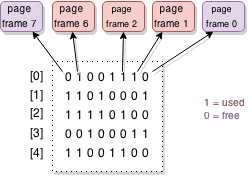
\includegraphics[scale=1]{figures/BitsMap}
	\caption{Beispiel einer Bitsmap zur Verwaltung der Page Frames}
	\label{fig:BitsMap}
\end{figure}

\subsection{Initialisierung der MMU}


\pagebreak 